\documentclass{beamer}

\mode<presentation> {
\usetheme{Malmoe} 
\usecolortheme{beaver} 
}

\usepackage{graphicx} 
\usepackage{booktabs} 
\usepackage{amsmath}
\usepackage{graphicx} %allows the following formats: .jpg  .png  .pdf  .mps
\graphicspath{{./figures/}} %Where the figures folder is located
\usepackage{media9}
\usepackage{verbatim}
\usepackage{ctable}
\usepackage{geometry}
%\geometry{verbose,letterpaper} %change page format
\usepackage[colorinlistoftodos]{todonotes}
\usepackage{hyperref}
\usepackage{multimedia}
\usepackage{multirow,tabularx}
\usepackage{tikz}
\usetikzlibrary{calc,positioning}
\usepackage{xcolor}
\hypersetup{
    colorlinks=true,       
    linkcolor=blue,          
    citecolor=blue,        
    urlcolor=blue           
}
\usepackage{multimedia}
%\usepackage{movie15}
%\newcommand{\fullpage}[1]{
%\begin{frame}
% #1
%\end{frame}
%}

%----------------------------------------------------------------------------------------
%	TITLE PAGE
%----------------------------------------------------------------------------------------

\title[CPS]{\textcolor{black}{{Integrated Online Perception of Articulated Objects for Manipulation \cite{p1}}}} 
\subtitle[]{}

\author{Jia Guo, George Kontoudis}
\institute[VT] 
{Semester Project\\
ME5524 Bayesian Robotics\\
Spring 2017\\
\medskip
\it{Mechanical Engineering Department, Virginia Tech} 
}
\date{\today}

\setbeamertemplate{footline}[text line]{%
  \parbox{\linewidth}{\vspace*{-8pt}\today 
  \hfill\insertshortsubtitle
  \hfill\insertpagenumber}}
\setbeamertemplate{navigation symbols}{}

\begin{document}

\begin{frame}[plain]
\titlepage 
\end{frame}

\begin{frame}
\frametitle{Outline} 
\scriptsize{\tableofcontents }
\end{frame}

%----------------------------------------------------------------------------------------
%	PRESENTATION SLIDES
%----------------------------------------------------------------------------------------
%------------------------------------------------
\section{Background}
%------------------------------------------------

\begin{frame}
\frametitle{Background}
\textbf{Problem:}
\begin{itemize}
\item Grasping and manipulation in unstructured environments 
\item Identify object's shape, pose, and kinematic structure 
\item Visual perception techniques cannot be solved online 
\end{itemize}
\vspace{.5cm}
\textbf{Solution:} 
\begin{itemize}
\item Utilization of Recursive Bayesian Estimation (RBE) techniques 
\item Allocation to sub-level algorithms 
\end{itemize}

\end{frame}

%------------------------------------------------
\section{Objective}
%------------------------------------------------

\begin{frame}
\frametitle{Objective} 
Identify kinematic structure of objects and environment w/ visual perception
\begin{itemize}
\item Estimate joint axis 
\item Estimate type of joints
\item Motion with uncertainty
\end{itemize}
\vspace{.5cm}
\textbf{Autonomous grasping in unstructured environment}


\end{frame}
%------------------------------------------------
\section{Motion \& Sensor Model}
%------------------------------------------------
\subsection{Kinematic Structure Estimation}

\begin{frame}
\frametitle{Kinematic Structure Identification}


\begin{columns}[c] % The "c" option specifies centered vertical alignment while the "t" option is used for top vertical alignment
\column{.62\textwidth} 
Estimation of kinematic structure using an RGB-D camera \vspace{.2cm}
\begin{enumerate}
\item The feature tracker is based on KLT algorithm \cite{p3}\vspace{.2cm}
\item Rigid body motion achieved w/ EKF\vspace{.2cm}
\item Kinematic model obtained w/ EKF
\end{enumerate}
   
\column{.54\textwidth} 
    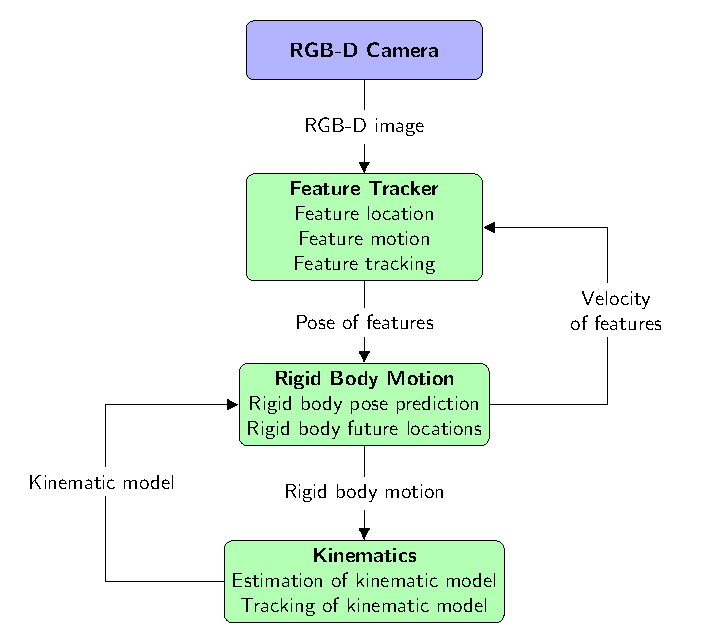
\includegraphics[scale=0.52]{RecursiveEstimation.pdf}
	\centering
\end{columns}

\end{frame}

%------------------------------------------------

\begin{frame}
\frametitle{Stochastic Models}
Motion model of EKF 
\begin{equation}
x_k^t=f^t(x_{k-1}^t,u_{k-1}^t)+w_{k-1}^t,
\end{equation} 
where $w_{k-1}^t \sim \mathcal{N}(0, \Sigma_{w_{k-1}^t})=\mathcal{N}(0, 
Q_{k-1})$, $Q_{k-1} \geq 0$\\
\vspace{.2cm}
Sensor model of EKF 
\begin{equation}\label{obsM}
z_{k-1}^t=h^t(x_{k-1}^t)+v_{k-1}^t,
\end{equation} 
where $v_{k-1}^t \sim \mathcal{N}(0, \Sigma_{v_{k-1}^t})=\mathcal{N}(0, R_{k-1})$ with $R_{k-1}>0$
\end{frame}

%------------------------------------------------
\subsection{Integrated Visual Perception}

\begin{frame}
\frametitle{Integrated Visual Perception}
Jia Guo
\end{frame}

%------------------------------------------------
\section{Developed Techniques}
%------------------------------------------------
\subsection{Developed Detection Techniques}

\begin{frame}
\frametitle{Developed/Implemented Detection Technique}
Jia Guo
\end{frame}

%------------------------------------------------
\subsection{Developed RBE Techniques}

\begin{frame}
\frametitle{RBE for Rigid Body Motion - 2$nd$ Level}
\textbf{Inputs}: Feature's pose (1$st$ level), Rigid body velocities (3$rd$ level) \\
\vspace{.4cm}
Sensor model of 2$nd$ level EKF 
\begin{equation}\label{obsMF}
z_k^t=h^t(x_{k-1}^t)+v_{k-1}^t= \begin{bmatrix}
T(p)f^1_{k-1} \\
\vdots \\
T(p)f^m_{k-1}
\end{bmatrix} + v_{k-1}^t,
\end{equation}
where $v_{k-1}^t \sim \mathcal{N}(0, \Sigma_{v_{k-1}^t})=\mathcal{N}(0, R_{k-1})$,  $R_{k-1}>0$, and $T(p)$ homogeneous transformation of the feature's pose\\
\vspace{.4cm}
\textbf{Output}: Rigid body motion (3$rd$ level)
\end{frame}
%------------------------------------------------

\begin{frame}
\frametitle{RBE for Kinematics Structure}
\textbf{Input}: Rigid body twist (2$nd$ level) \\
\vspace{.4cm}
Sensor model of 3$rd$ level EKF for prismatic joints
\begin{equation}
z_{pr, joint}^t=\begin{bmatrix}
q_p \hat{o}_p\\
0_3 
\end{bmatrix} + v_{k-1}^t,
\end{equation}

\vspace{.2cm}
Sensor model of 3$rd$ level EKF for revolute joints
\begin{equation}
z_{rev, joint}^t=\begin{bmatrix}
(-q_r \hat{o}_r) \times p_r\\
q_r \hat{o}_r
\end{bmatrix} + v_{k-1}^t,
\end{equation}

\vspace{.4cm}
\textbf{Output}: Kinematic Model (2$nd$ level)
\end{frame}
%------------------------------------------------
\section{Simulations and Experiments}
%------------------------------------------------
\subsection{Implementation in ROS}
\begin{frame}
\frametitle{Implementation in ROS}
\begin{itemize}
\item Simulations and experiments were conducted in ROS
\item With .bag files we check the validity of the proposed methodology 
\item RGB-D stream utilized for experimental kinematic structure identification
\item Uncertainty of the estimation is also studied
\end{itemize}
\includegraphics[scale=0.23]{cover.png}
	\centering

\end{frame}

%------------------------------------------------
\begin{frame}
\frametitle{ROS Computation Graph}
\begin{columns}[c]
\column{.78\textwidth} 
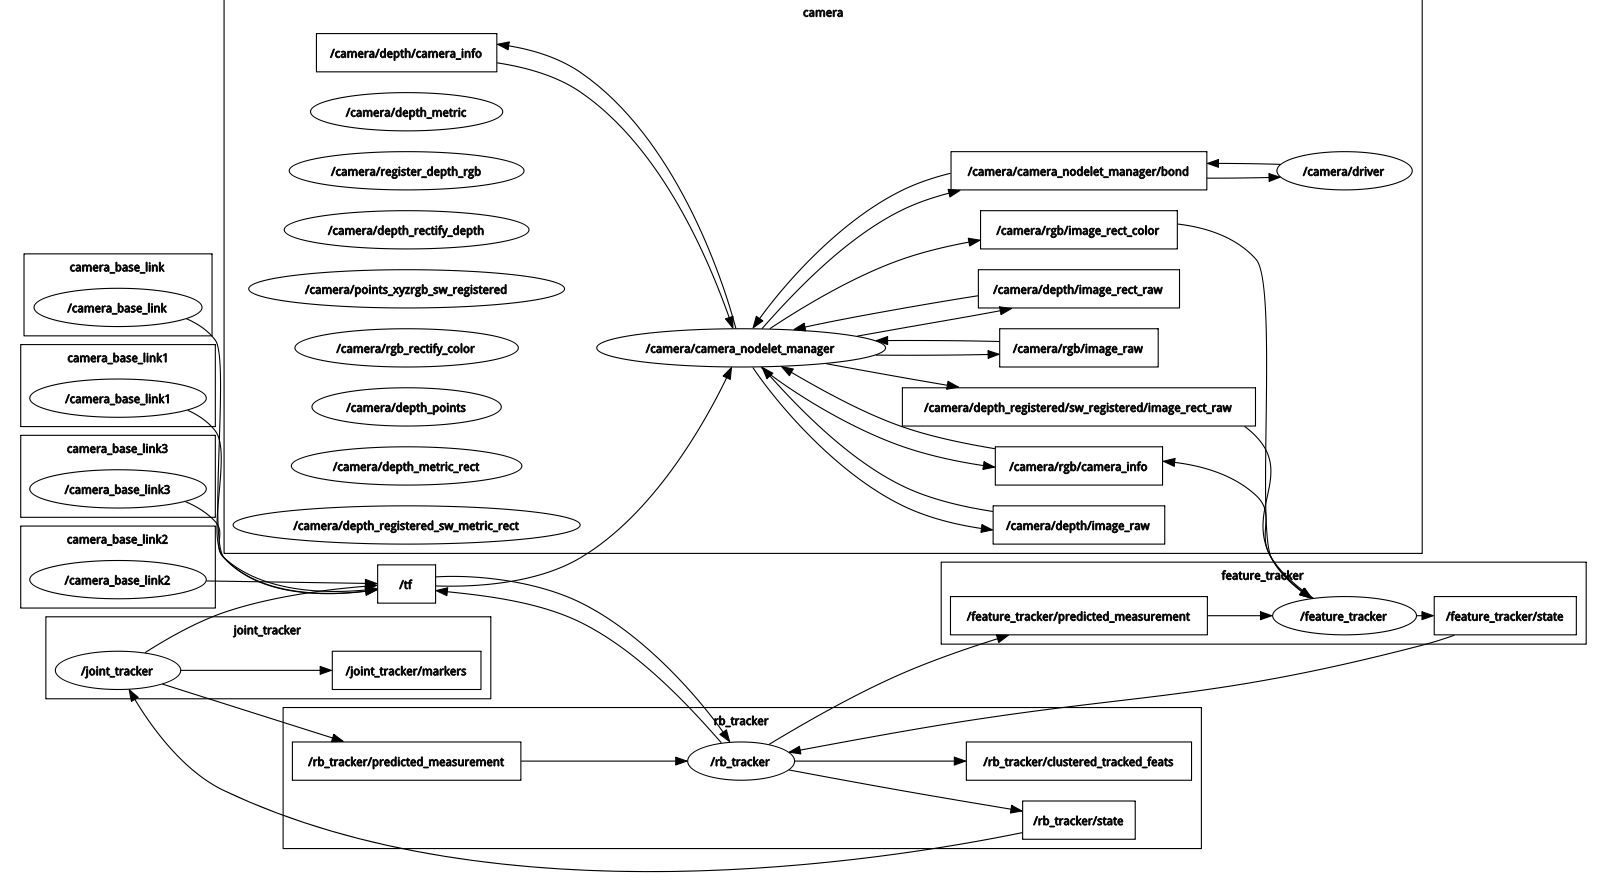
\includegraphics[scale=0.25]{rqt_graph.png}

\column{.38\textwidth}
\begin{itemize}
\item \textbf{RGB-D camera}
\item \textbf{Feature tracker}\\
I: RGB-D image
\item \textbf{Rigid body motion}\\
I: Feature's velocity\\
O: Pose of features
\item \textbf{Kinematics}\\
I: RB motion\\
O: Kinematic model
\end{itemize}
\end{columns}
\end{frame}

%------------------------------------------------
\subsection{Experiments with an RGB-D Camera}
\begin{frame}
\frametitle{Experiments}
%\includemedia[
%  width=0.6\linewidth,height=0.45\linewidth,
%  activate=pageopen,
%  flashvars={
%    modestbranding=1 % no YT logo in control bar
%   &autohide=1       % controlbar autohide
%   &showinfo=0       % no title and other info before start
%  }
%%]{}{https://youtu.be/weG94fqyQpY}   % Flash file  
%]{}{http://www.youtube.com/v/weG94fqyQpY?rel=0}   % Flash file
%%\fullpage{See Demo video}
%%\includemovie[poster,autoplay,externalviewer, text={\small(Loading bloch.mp4)}]{6cm}{6cm}{figures/BayesianRobotics_KontoudisGuo.mp4}
%%\movie[width=3cm,height=2cm,poster]{}{figures/BayesianRobotics_KontoudisGuo.mp4}
%\movie[height = 0.6\textwidth, width = 0.8\textwidth, poster, showcontrols] {}{BayesianRobotics_KontoudisGuo.mp4}
\begin{center}
\url{https://youtu.be/weG94fqyQpY}
\end{center}
\end{frame}


%------------------------------------------------
\section{Conclusions and Future Work}
%------------------------------------------------

\begin{frame}
\frametitle{Conclusions and Future Work}

Conclusions
\begin{itemize}
\item Method is valid for online kinematic structure identification 
\item Includes 3 sub-level recursive estimation models
\item Shape-based tracker to refine the outcomes of feature tracker 
\item Simulations and experiments conducted

\end{itemize}
\vspace{.4cm}

Future Work
\begin{itemize}
\item Utilization of contemporary ft (KLT \cite{p3})
\item UKF instead of EKF might provide better results
\item Incorporate online perception technique to our robots 
\end{itemize}


\end{frame}

%------------------------------------------------


%------------------------------------------------
\section{References}
%------------------------------------------------
\begin{frame}
\frametitle{References}
\scriptsize{
\begin{thebibliography}{99} % Beamer does not support BibTeX so references must be inserted manually as below

\bibitem[Martin, 2014]{p1} R. Martin and O. Brock (2014)
\newblock Online interactive perception of articulated objects with multi-level recursive estimation based on task-specific priors
\newblock \emph{IEEE/RSJ International Conference on Intelligent Robots and Systems (IROS), 2494-2501}, 2014.

\bibitem[Martin, 2016]{p2} R. Martin, S. H{\"o}fer and O. Brock (2016)
\newblock An integrated approach to visual perception of articulated objects
\newblock \emph{IEEE International Conference on Robotics and Automation (ICRA), 5091--5097}, 2016.

\bibitem[Tomasi, 1991]{p3} C. Tomasi and T. Kanade (1991)
\newblock Detection and tracking of point features
\newblock \emph{Technical Report, CMU-CS-91-132}, 1991.


\end{thebibliography}
}
\end{frame}

%------------------------------------------------
\section{}
\begin{frame}
\begin{center}
\Huge {Thank You!}
\end{center}
\end{frame}

%----------------------------------------------------------------------------------------

\end{document} 